\documentclass[12pt]{article}
\usepackage[utf8]{inputenc}
\usepackage{amsmath}
\usepackage{amsfonts}
\usepackage{graphicx}
\usepackage[backend=biber, style=apa]{biblatex}
\addbibresource{Bibliography.bib} 
\usepackage{hyperref}
\usepackage[spanish]{babel}
\usepackage{csquotes} % para citas adecuadas
\DeclareLanguageMapping{spanish}{spanish-apa} % mapeo del idioma

\begin{document}
	\begin{titlepage}
		  \centering
		 
		  
		  {\scshape\LARGE Facultad de Matemática y 
		  	Computación
		  	Universidad de La Habana\par}
		  \vspace{1cm}
		  
		   %\includegraphics[width=0.15\textwidth]{logo_universidad} % Logo de la universidad
		   \vspace{1cm}
		  
		  {\scshape\Large Tesis de diploma de la 
		  	Especialidad Ciencia de la 
		  	Computaci\'on \par}
		  \vspace{1.5cm}
		  
		  {\huge\bfseries Segmentaci\'on de \'Ulceras de Pie Diab\'etico (UPD) en secuencias de im\'agenes RGB mediante el Segment Anything Model (SAM). \par}
		  \vspace{2cm}
		  
		  {\Large Autor: Abdel Fregel Hern\'andez \par}
		  
		  \Large Tutor: Dr. Jos\'e Alejandro Mesejo Chiong
		  \vfill
		  
		  {\large La Habana}
		  
		  {\large \today \par} % Fecha actual
	\end{titlepage}
	
	\section{Agradecimientos}
	\pagenumbering{roman}
	\newpage
	
	
	\section{Resumen}
	\newpage
	
	\section{\'Indice}
	\tableofcontents
	\newpage
	\cleardoublepage
	\pagenumbering{arabic}
	
	
	\section{Introducci\'on}
	La diabetes(diabetes mellitus), es una enfermedad cr\'onica que afecta la forma en la que el cuerpo utiliza la glucosa, una fuente clave de energ\'ia. De acuerdo a la \textit{Federaci\'on Internacional de Diabetes}, en el a\~no 2021 se reportaron 6.7 millones de muertes a causa de esta enfermedad \parencite{DiabetesAtlas2024}. En nuestro pa\'is, seg\'un el \textit{Anuario Estadístico de Salud 2022} \parencite{msp2022}, la prevalencia es de 66,50\textdiscount \space de enfermos por cada 1000 habitantes.
	\\
	
	Cerca del 86\textdiscount \space de personas que padecen de diabetes sufren de \'ulcera de pie diab\'etico \footnote{Hace referencia a una complicaci\'on grave de la diabetes que se manifiesta como una herida o llaga abierta en el pie}(UPD), y corren el riesgo de amputaci\'on. La cicatrizaci\'on de estas \'ulceras puede tardar semanas, meses e incluso a\~nos, deteriorando la calidad de vida de los pacientes. Actualmente, los médicos cubanos especializados en el tema no cuentan con una herramienta cuantitativa efectiva que valore la severidad y el proceso de curación de las UPD. La medición regular de las úlceras es crucial para evaluar la efectividad del tratamiento y realizar ajustes cuando sea necesario. Un seguimiento adecuado puede prevenir la progresión de la úlcera y reducir el riesgo de amputaciones.
	\\
	
	
	Existen m\'etodos de segmentaci\'on y medici\'on de heridas que han conseguido grandes avances en esta \'area. La calidad de estas es esencial para varios an\'alisis de heridas, como por ejemplo la clasificaci\'on de tejidos, Reconstrucci\'on 3D, y la evaluaci\'on de la cicatrizaci\'on\parencite{Filko2023}. Se pueden clasificar en dos tipos: aquellos que requieren contacto y los que no. Los métodos de contacto son invasivos y presentan un alto margen de error; por ello, este trabajo se centra en los métodos no invasivos.
	\\
	
	 

	
	Varios estudios han abordado esta problem\'atica. Por ejemplo, en \parencite{Filko2023} hacen uso de un sofisticado brazo rob\'otico de 7 grados de libertad(DoF), equipado con una c\'amara RGB-D \footnote{RGB-D, se refiere a una camara capaz de captar im\'agenes a color(RGB, formato Red(rojo),Green(verde),Blue(\'azul) y un sensor de profundidad (D(depth),por su sigla en ingl\'es)} y un esc\'aner 3D de alta precisi\'on, para la segmentaci\'on y medici\'on de heridas. Este artículo aporta un nuevo algoritmo de segmentación que utiliza una combinación de procedimientos 2D y 3D para segmentar correctamente un modelo de herida en 3D. La segmentación se realiza a partir de múltiples fotografías 2D por herida, impulsada por una red neuronal profunda en forma del clasificador MobileNetV2 \parencite{Filko2023}. Este clasificador se combina óptimamente con un único modelo 3D y la inicialización del contorno de la herida. Este contorno inicial se optimiza y ajusta mediante un modelo de contorno activo \parencite{Filko2023}, que envuelve estrechamente la superficie real de la herida utilizando la curvatura de la superficie para alcanzar su objetivo.
	\\
	
	En otro estudio realizado por \cite{Filko2018} se explor\'o la medici\'on y reconstrucci\'on de heridas cr\'onicas de lenta curaci\'on, ultilizando c\'amara RGB-D. Con la llegada de cámaras RGB-D económicas, la comunidad de visión por computadora ha ganado una forma más accesible para innovar y crear aplicaciones en diversos campos, incluyendo la medicina, \cite{Filko2018}. Estas cámaras, que combinan información de color y profundidad, permiten un análisis más detallado y preciso de imágenes, facilitando el desarrollo de tecnologías que mejoran diagnósticos y tratamientos. El sistema desarrollado en dicho art\'iculo detecta automáticamente heridas analizando bloques de imagen según la similitud del histograma de color utilizando un enfoque de vecinos más cercanos(KNN,por sus siglas en \'ingles). Este método permite identificar características específicas de las heridas en imágenes, facilitando su segmentación y medición.
	\\
	
	Es fundamental el desarrollo de una herramienta capaz de realizar la segmentaci\'on y la medici\'on de estas heridas lo m\'as preciso posible, por lo que en este trabajo se propone , para la tarea de segmentar las im\'agenes,  utilizar una herramienta desarrollada por Meta AI llamada Segment Anything Model(SAM)\parencite{segmentanything2023} que permite identificar y segmentar objetos en imágenes de manera eficiente. Esta herramienta ha ganado popularidad en cuanto a las tareas de segmentaci\'o y en el presente trabajo ser\'a usada para hacer una segmentaci\'on de las imagenes de UPD, las cuales ser\'an tomadas con una c\'amara RGB-D para asegurar su calidad.
	\\
	
	 La c\'amara que se utiliza es una c\'amara Intel Realsense D435i RGB-D. La cámara utiliza luz estructurada infrarroja y métodos binoculares para obtener información de profundidad, que es la tecnología más común y madura utilizada en las cámaras RGB-D de grado consumidor actuales. La cámara de profundidad puede emitir un flujo de video de hasta 720p a 90 FPS, y la cámara RGB puede emitir un flujo de video de hasta 1080p a 30 FPS \parencite{Zhang2023}. Luego de la segmentaci\'on se realizar\'a una clasificaci\'on de los tejidos para poder realizar una evaluaci\'on de la cicatrizaci\'on.
	 \\
	 
	La importancia de los tejidos en el proceso de cicatrización radica en que cada tipo de tejido desempeña un papel crucial en la reparación y regeneración de la herida. Durante la cicatrización, se forman diferentes tipos de tejidos, siendo el tejido de granulación uno de los más fundamentales \parencite{CUN2023}. Este tejido no solo es esencial para el cierre de la herida, sino que también prepara el lecho para la epitelización, proporcionando un entorno adecuado para la migración celular y la formación de nuevos vasos sanguíneos.
	
	Sin embargo, la presencia de tejido necrótico y biofilm bacteriano puede complicar este proceso. El tejido necrótico, formado por células muertas y detritos, actúa como una barrera que impide la formación de tejido de granulación saludable \parencite{Ulceras2024}. Esto no solo retrasa el proceso de curación, sino que también aumenta el riesgo de infección, lo que puede llevar a complicaciones graves, como la amputación. Por lo tanto, es crucial realizar un desbridamiento adecuado para remover el tejido necrótico y permitir que la herida progrese hacia las fases de proliferación y cicatrización.
	Por otro lado, el biofilm bacteriano se forma cuando microorganismos se adhieren a la superficie del lecho de la herida, creando microcolonias protegidas por una matriz polimérica. Esta estructura no solo protege a las bacterias de los tratamientos antibióticos convencionales, sino que también interfiere con la respuesta inmune del cuerpo y dificulta la migración celular necesaria para regenerar tejido sano. La identificación y tratamiento adecuados del tejido necrótico y el biofilm son esenciales para facilitar una curación efectiva y mejorar la calidad de vida del paciente.
	
	\subsection{Objetivos}
	Este trabajo tiene como objetivo desarrollar una herramienta que permita realizar la segmentación automática de úlceras y los tejidos que las componen a partir de una secuencia de imágenes RGB-D, facilitando así el tratamiento por parte del médico.	
	\\
	
	
	Para lograr este objetivo general se tiene los siguientes objetivos espec\'ificos:
	
	\begin{itemize}
		\item[1] Hacer un estudio de la literatura sobre los m\'etodos de segmentaci\'on
		\item[2] Estudiar sobre la utilizaci\'on del Segment Anything Model.
		\item[3] La creaci\'on de un dataset para la posterior evaluaci\'on del modelo
		\item[4] La evaluaci\'on del modelo en cuanto m\'etricas de calidad. 
	\end{itemize}
	
	\subsection{Estructura de la tesis}
	La tesis está organizada en cuatro capítulos. El Capítulo 1 presenta una revisión literaria donde se discuten algunos algoritmos existentes así como datasets relevantes. El Capítulo 2 ofrece una introducción al SAM y su aplicación en imágenes médicas. En el Capítulo 3 se explican los detalles estructurales e implementativos del sistema propuesto. Finalmente, el Capítulo 4 muestra los resultados obtenidos y compara estos con otros modelos existentes utilizando medidas cualitativas. Se concluirá con recomendaciones basadas en esta investigación para futuras continuaciones del trabajo. Esta versión busca mantener un hilo conductor claro entre las ideas expuestas, eliminando saltos innecesarios y mejorando la cohesión general del texto.

	
	
	
	\newpage
	
	\section{Cap\'itulo 1}
		\subsection{Estado del arte}
	
	
	\newpage
	
	\section{Cap\'itulo 2}
		\subsection{Segment Anything Model(SAM)}
		SAM utiliza una arquitectura transformer-based,a la cual se le ha probado su eficiencia en el procesamiento de lenguaje natural y en tareas de reconocimiento de im\'agenes. Espec\'ificamente, SAM contiene un codificador de imagen(image encoder) basado en un Vision Transformer(ViT), con este extrae las caracter\'isticas de la imagen, tambi\'en utiliza un prompt encoder para integrar las interacciones del usuario y por \'ultimo un mask decoder con el objetivo de predecir las m\'ascaras de segmentaci\'on con la fusi\'on de las caracter\'isticas de la imagen con las entradas del usuario.
		\\
		
		En la figura \ref{fig:fig1} se aprecia la estructura de SAM:
		\begin{itemize}
			\item[1] Image Encoder: SAM utiliza un image encoder basado en un Vision Transformer  preentrenado en el esquema de Masked Autoencoder(MAE), el cual esta adaptado para procesar im\'agenes de alta resoluci\'on. Este toma im\'agenes de 1024 x 1024 y da como salida image embeddings bajando su tama\~no a un mapa de caracter\'isticas de 64 x 64.
			\item[2] Prompt Encoder: para esto dos tipos de ellos son considerados, uno incluyendo puntos y rect\'angulos y otro que trabaja con m\'ascaras.
			
			\item[3] Mask Decoder : consiste en dos transformer layers con una m\'ascara de predicci\'on din\'amica y  una puntuaci\'on de regresi\'on Intersection-over-Union(IoU, por sus siglas en \'ingles)
		\end{itemize}
		
		\begin{figure}[h] 
			\centering
			\caption{ Imagen adaptada de}
			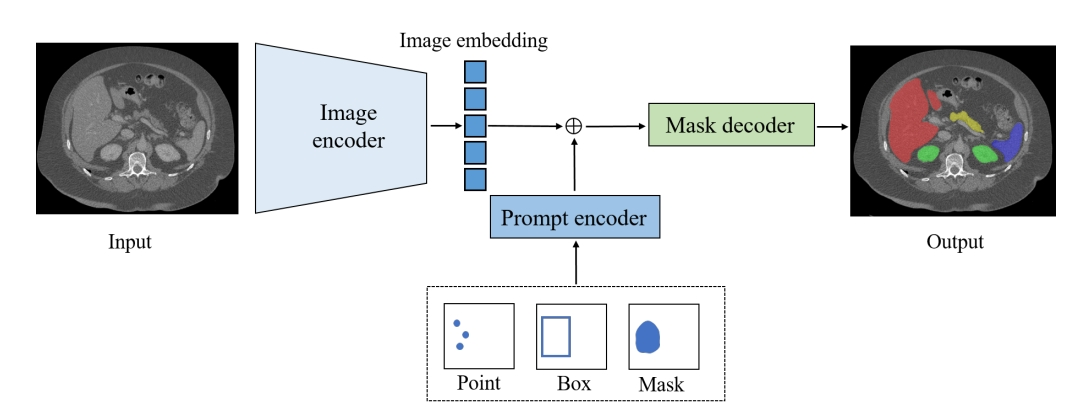
\includegraphics[width=1\textwidth]{1.jpeg}
			
			\label{fig:fig1}
			
			
		\end{figure}
	
	\newpage
	
	\section{Conclusiones}
	\newpage
	
	\section{Recomendaciones}
	en la figura \ref{fig:fig1}
	\newpage
	
	\section{Bibliograf\'ia}
	\printbibliography[title={" "}]
	\newpage
	
	\section{Anexos}
	
	
\end{document}